\documentclass{article}


\usepackage{amsmath,amssymb,amsthm,amsfonts,amscd}
\usepackage{multirow}
\usepackage{animate}
\usepackage{bbm}
\usepackage{enumerate}
\usepackage[tmargin=1in, bmargin=1in, lmargin=0.75in, rmargin=0.75in]{geometry}
\usepackage[colorlinks]{hyperref}
\usepackage{mathtools}
\usepackage[framemethod=tikz]{mdframed}
\usepackage{doi}
\usepackage{framed}
\usepackage{xcolor}
\usepackage{graphicx}
\usepackage{mathrsfs}
\usepackage{esvect}
\usepackage{commath}
\usepackage{lastpage}
\usepackage{mathpazo}
% \usepackage{tgpagella}
\usepackage{anyfontsize}
\usepackage{tkz-graph}
\usepackage[linesnumbered,ruled,vlined]{algorithm2e}
\usepackage[capitalize, nameinlink]{cleveref}
\newcommand\mycommfont[1]{\footnotesize\ttfamily{#1}}
\SetCommentSty{mycommfont}
\SetArgSty{textup}
\usepackage[square,numbers]{natbib}
\usepackage{verbatim}
\usepackage{titlesec}
\titleformat{\section}[block]{\sffamily\Large\filcenter\bfseries}{\S\thesection.}{0.25cm}{\Large}
\titleformat{\subsection}[block]{\large\bfseries\sffamily}{\thesubsection.}{0.2cm}{\large}
\titleformat{\subsubsection}[block]{\large\bfseries\sffamily}{\normalsize\thesubsubsection.}{0.15cm}{\normalsize}
\usepackage{listings} % For code listings

\colorlet{shadecolor}{black}
\lstnewenvironment{code}{%
\footnotesize
    \shaded
    \lstset{
        basicstyle=\ttfamily\color{white},
        backgroundcolor=\color{shadecolor},
        frame=single, % Add a frame around the code
        framerule=0pt, % No rule width for the frame
        framesep=4pt, % Adjust the spacing between frame and content
    }%
}{%
    \endshaded
}

\usepackage{fancyhdr}
% \renewcommand\thesubsection{\thesection.\alph{subsection}}

\Crefname{algocf}{Algorithm}{Algorithms}


\newcommand{\hr}[1]{\rule{\linewidth}{#1}}



\title{COL334 Assignment1}
\author{Ankit Mondal and Anish Banerjee}
\begin{document}
\maketitle

\section{Network Analysis}
\begin{enumerate}[a.]
    \item We ran {\tt tracert} on {\tt iitd.ac.in} outside IITD network and got the following output:
    \begin{code}
PS C:\Users\Anish> tracert iitd.ac.in

Tracing route to iitd.ac.in [103.27.9.24]
over a maximum of 30 hops:

 1    4 ms    3 ms    9 ms dsldevice.lan [192.168.1.1]
 2   87 ms   73 ms   26 ms abts-north-dynamic-255.187.69.182.airtelbroadband.in [182.69.187.255]
 3   34 ms   28 ms   48 ms 125.18.240.153
 4   38 ms   45 ms   38 ms 116.119.106.136
 5   47 ms   53 ms   49 ms 49.44.220.188
 6    *       *       *    Request timed out.
 7    *       *       *    Request timed out.
 8   47 ms   43 ms   47 ms 136.232.148.178
 9    *       *       *    Request timed out.
10    *       *       *    Request timed out.
11    *       *       *    Request timed out.
12   45 ms   59 ms   52 ms 103.27.9.24
13  187 ms   46 ms   61 ms 103.27.9.24
14   47 ms   48 ms   49 ms 103.27.9.24

Trace complete.
    \end{code}
    \item TODO
    \item We observe that the maximum packet size that can be sent is 68 (to {\tt google.com})
\begin{code}
root@IdeapadAB:/mnt/c/Users/Anish# ping -s 68 -c 5 google.com
PING google.com (142.250.194.238) 68(96) bytes of data.
76 bytes from del12s08-in-f14.1e100.net (142.250.194.238): icmp_seq=1 ttl=116 time=7.00 ms
76 bytes from del12s08-in-f14.1e100.net (142.250.194.238): icmp_seq=2 ttl=116 time=6.73 ms
76 bytes from del12s08-in-f14.1e100.net (142.250.194.238): icmp_seq=3 ttl=116 time=7.11 ms
76 bytes from del12s08-in-f14.1e100.net (142.250.194.238): icmp_seq=4 ttl=116 time=6.05 ms
76 bytes from del12s08-in-f14.1e100.net (142.250.194.238): icmp_seq=5 ttl=116 time=7.98 ms

--- google.com ping statistics ---
5 packets transmitted, 5 received, 0% packet loss, time 4007ms
rtt min/avg/max/mdev = 6.052/6.973/7.975/0.621 ms
root@IdeapadAB:/mnt/c/Users/Anish# ping -s 69 -c 5 google.com
PING google.com (142.250.194.238) 69(97) bytes of data.

--- google.com ping statistics ---
5 packets transmitted, 0 received, 100% packet loss, time 4009ms  
\end{code}
However, we also observe that the max ping size depends on the site requested for. For example, we saw that for {\tt iitd.ac.in}, it is 1472 bytes.
We can run the following python code to find the maximum packet size for a given site:
\begin{code}
    #!/usr/bin/python3

    import os
    site=input("Enter the site: ")
    l=1
    r=65007
    while l<r:
        mid=(l+r)//2
        if os.system("ping -c 1 -s "+str(mid)+" "+site)==0:
            l=mid+1
        else:
            r=mid
    print("\n\nMax ping size is: "+str(l-1))
\end{code}
\end{enumerate}

\section{{\tt traceroute} using python}
The code for {\tt traceroute} can be found in {\tt traceroute.py}. 

\section{Internet Architecture}

First we run a traceroute from our own IP address to the 5 different servers.

\begin{enumerate}[a.]

\item Here is the route to {\tt www.google.com}
\begin{code}
Ankits-MacBook-Air-6:~ ankitmondal$ traceroute google.com
traceroute to google.com (142.250.194.238), 64 hops max, 52 byte packets
 1  10.184.0.13 (10.184.0.13)  3.999 ms  3.570 ms  3.506 ms
 2  10.254.175.1 (10.254.175.1)  4.146 ms
    10.254.175.5 (10.254.175.5)  3.675 ms  3.223 ms
 3  10.255.1.34 (10.255.1.34)  3.562 ms  3.512 ms  3.357 ms
 4  10.119.233.65 (10.119.233.65)  3.463 ms  3.959 ms  3.930 ms
 5  * * *
 6  10.119.234.162 (10.119.234.162)  12.045 ms  5.639 ms  5.675 ms
 7  72.14.194.160 (72.14.194.160)  5.484 ms  5.647 ms  6.487 ms
 8  108.170.251.113 (108.170.251.113)  7.106 ms
    108.170.251.97 (108.170.251.97)  6.339 ms  6.480 ms
 9  142.251.52.217 (142.251.52.217)  6.274 ms  6.749 ms  6.689 ms
10  del12s08-in-f14.1e100.net (142.250.194.238)  6.588 ms  6.423 ms  6.608 ms
\end{code}

\item Here is the route to {\tt www.iitd.ac.in}
\begin{code}
Ankits-MacBook-Air-6:~ ankitmondal$ traceroute www.iitd.ac.in
traceroute to www.iitd.ac.in (10.10.211.212), 64 hops max, 52 byte packets
 1  10.184.0.13 (10.184.0.13)  4.675 ms  4.242 ms  3.512 ms
 2  10.254.175.5 (10.254.175.5)  4.012 ms
    10.254.175.1 (10.254.175.1)  4.016 ms  4.356 ms
 3  10.254.236.6 (10.254.236.6)  3.285 ms
    10.254.236.26 (10.254.236.26)  3.920 ms
    10.254.236.2 (10.254.236.2)  5.730 ms
 4  www.iitd.ac.in (10.10.211.212)  3.830 ms  4.643 ms  5.628 ms
 \end{code}
 \item Here is the route to {\tt www.utah.edu}
 
\begin{code}
Ankits-MacBook-Air-6:~ ankitmondal$ traceroute www.utah.edu
traceroute to www.utah.edu (155.98.186.21), 64 hops max, 52 byte packets
 1  10.184.0.13 (10.184.0.13)  5.480 ms  3.898 ms  3.338 ms
 2  10.254.175.1 (10.254.175.1)  3.602 ms
    10.254.175.5 (10.254.175.5)  3.922 ms  3.769 ms
 3  10.255.1.34 (10.255.1.34)  5.116 ms  5.269 ms  5.756 ms
 4  10.119.233.65 (10.119.233.65)  64.339 ms  67.830 ms  65.010 ms
 5  10.1.207.69 (10.1.207.69)  80.742 ms  86.632 ms  93.759 ms
 6  10.1.200.137 (10.1.200.137)  84.119 ms  85.695 ms  70.847 ms
 7  10.255.238.254 (10.255.238.254)  80.166 ms
    10.255.238.122 (10.255.238.122)  78.281 ms
    10.255.238.254 (10.255.238.254)  86.918 ms
 8  180.149.48.18 (180.149.48.18)  71.995 ms  60.372 ms  58.199 ms
 9  180.149.48.6 (180.149.48.6)  244.512 ms  207.941 ms  197.721 ms
10  180.149.48.20 (180.149.48.20)  182.712 ms
    180.149.48.13 (180.149.48.13)  337.379 ms
    180.149.48.20 (180.149.48.20)  173.159 ms
11  fourhundredge-0-0-0-2.4079.core1.ashb.net.internet2.edu (163.253.1.116)  340.584 ms
    180.149.48.13 (180.149.48.13)  270.570 ms
    fourhundredge-0-0-0-2.4079.core1.ashb.net.internet2.edu (163.253.1.116)  314.143 ms
12  fourhundredge-0-0-0-16.4079.core2.ashb.net.internet2.edu (163.253.1.3)  312.121 ms
    fourhundredge-0-0-0-2.4079.core1.ashb.net.internet2.edu (163.253.1.116)  417.111 ms
    fourhundredge-0-0-0-16.4079.core2.ashb.net.internet2.edu (163.253.1.3)  416.768 ms
13  fourhundredge-0-0-0-16.4079.core2.ashb.net.internet2.edu (163.253.1.3)  313.367 ms
    fourhundredge-0-0-0-1.4079.core2.clev.net.internet2.edu (163.253.1.139)  319.440 ms  418.102 ms
14  fourhundredge-0-0-0-1.4079.core2.clev.net.internet2.edu (163.253.1.139)  417.208 ms
    fourhundredge-0-0-0-2.4079.core2.eqch.net.internet2.edu (163.253.2.17)  416.394 ms
    fourhundredge-0-0-0-1.4079.core2.clev.net.internet2.edu (163.253.1.139)  319.361 ms
15  fourhundredge-0-0-0-2.4079.core2.eqch.net.internet2.edu (163.253.2.17)  410.326 ms
    fourhundredge-0-0-0-2.4079.core2.chic.net.internet2.edu (163.253.2.18)  416.659 ms
    fourhundredge-0-0-0-2.4079.core2.eqch.net.internet2.edu (163.253.2.17)  417.562 ms
16  fourhundredge-0-0-0-2.4079.core2.chic.net.internet2.edu (163.253.2.18)  415.580 ms  417.440 ms
    fourhundredge-0-0-0-1.4079.core1.kans.net.internet2.edu (163.253.1.245)  418.242 ms
17  fourhundredge-0-0-0-1.4079.core1.kans.net.internet2.edu (163.253.1.245)  418.728 ms
    fourhundredge-0-0-0-1.4079.core1.denv.net.internet2.edu (163.253.1.242)  416.527 ms  417.077 ms
18  fourhundredge-0-0-0-1.4079.core1.denv.net.internet2.edu (163.253.1.242)  416.455 ms
    fourhundredge-0-0-0-3.4079.core1.salt.net.internet2.edu (163.253.1.171)  418.388 ms
    fourhundredge-0-0-0-1.4079.core1.denv.net.internet2.edu (163.253.1.242)  314.445 ms
19  fourhundredge-0-0-0-3.4079.core1.salt.net.internet2.edu (163.253.1.171)  315.540 ms
    fourhundredge-0-0-0-1.4079.core1.lasv.net.internet2.edu (163.253.1.152)  411.072 ms
    fourhundredge-0-0-0-3.4079.core1.salt.net.internet2.edu (163.253.1.171)  417.062 ms
20  163.253.5.7 (163.253.5.7)  319.476 ms  319.171 ms
    fourhundredge-0-0-0-1.4079.core1.lasv.net.internet2.edu (163.253.1.152)  410.432 ms
21  tdc-beibr-b-170-int.uen.net (140.197.249.81)  415.347 ms  322.845 ms  404.272 ms
22  tdc-beibr-b-170-int.uen.net (140.197.249.81)  363.062 ms
    ddc-pep-c-123-int.uen.net (140.197.251.32)  318.119 ms
    tdc-beibr-b-170-int.uen.net (140.197.249.81)  322.820 ms
23  ddc-pep-c-123-int.uen.net (140.197.251.32)  346.374 ms
    ddc-pep-b-129-int.uen.net (140.197.253.97)  416.809 ms
    ddc-pep-c-123-int.uen.net (140.197.251.32)  411.102 ms
24  ddc-pep-b-129-int.uen.net (140.197.253.97)  416.736 ms
    ebc-pep-b-179-int.uen.net (140.197.252.76)  416.798 ms
    ddc-pep-b-129-int.uen.net (140.197.253.97)  412.609 ms
25  ebc-pep-a-178-int.uen.net (140.197.252.84)  416.708 ms  411.943 ms
    ebc-pep-b-179-int.uen.net (140.197.252.76)  419.376 ms
26  * ebc-pep-a-178-int.uen.net (140.197.252.84)  319.891 ms *
27  * 199.104.93.22 (199.104.93.22)  337.648 ms *
28  199.104.93.22 (199.104.93.22)  321.654 ms
    199.104.93.29 (199.104.93.29)  343.305 ms
    199.104.93.22 (199.104.93.22)  345.169 ms
\end{code}
\begin{code}
29  155.99.130.57 (155.99.130.57)  416.730 ms
    199.104.93.29 (199.104.93.29)  416.822 ms  416.541 ms
30  155.99.130.103 (155.99.130.103)  414.959 ms
    155.99.130.57 (155.99.130.57)  313.681 ms
    155.99.130.107 (155.99.130.107)  416.673 ms
31  172.31.241.255 (172.31.241.255)  416.605 ms
    155.99.130.101 (155.99.130.101)  412.722 ms
    172.31.241.255 (172.31.241.255)  416.726 ms
32  172.31.241.255 (172.31.241.255)  416.528 ms *
    172.31.241.251 (172.31.241.251)  423.757 ms
33  172.31.241.25 (172.31.241.25)  413.229 ms  404.049 ms
    172.31.241.22 (172.31.241.22)  425.597 ms
34  www.utah.edu (155.98.186.21)  412.101 ms * *
\end{code}

\item Here is the route to {\tt www.facebook.com}
\begin{code}
Ankits-MacBook-Air-6:~ ankitmondal$ traceroute facebook.com
traceroute to facebook.com (157.240.16.35), 64 hops max, 52 byte packets
 1  10.184.0.13 (10.184.0.13)  4.151 ms  3.441 ms  3.988 ms
 2  10.254.175.5 (10.254.175.5)  3.479 ms
    10.254.175.1 (10.254.175.1)  3.745 ms  3.525 ms
 3  10.255.1.34 (10.255.1.34)  3.845 ms  3.429 ms  6.735 ms
 4  10.119.233.65 (10.119.233.65)  13.776 ms  5.528 ms  4.366 ms
 5  10.1.207.69 (10.1.207.69)  29.882 ms  30.418 ms  31.270 ms
 6  * * *
 7  10.255.238.122 (10.255.238.122)  39.404 ms
    10.255.238.254 (10.255.238.254)  34.321 ms
    10.255.238.122 (10.255.238.122)  32.331 ms
 8  10.152.7.214 (10.152.7.214)  35.129 ms  33.873 ms  35.280 ms
 9  10.152.7.233 (10.152.7.233)  29.310 ms
    ae1.pr01.bom1.tfbnw.net (157.240.68.238)  53.885 ms  35.890 ms
10  po101.psw01.bom1.tfbnw.net (31.13.29.205)  38.635 ms
    po101.psw02.bom1.tfbnw.net (157.240.33.239)  35.706 ms
    ae2.pr02.bom1.tfbnw.net (157.240.66.204)  30.943 ms
11  po101.psw04.bom1.tfbnw.net (157.240.44.31)  29.498 ms *
    po102.psw02.bom1.tfbnw.net (157.240.35.63)  39.553 ms
12  157.240.38.65 (157.240.38.65)  30.149 ms
    173.252.67.185 (173.252.67.185)  35.504 ms
    edge-star-mini-shv-01-bom1.facebook.com (157.240.16.35)  31.092 ms
\end{code}
\end{enumerate}

\clearpage
\section{Packet Analysis}
\begin{enumerate}[a.]
    \item We ran a DNS filter on the output to {\tt iitd.ac.in} and got the following result(\cref{fig:IITDDNS}):
    \begin{figure}[!ht]
        \centering
        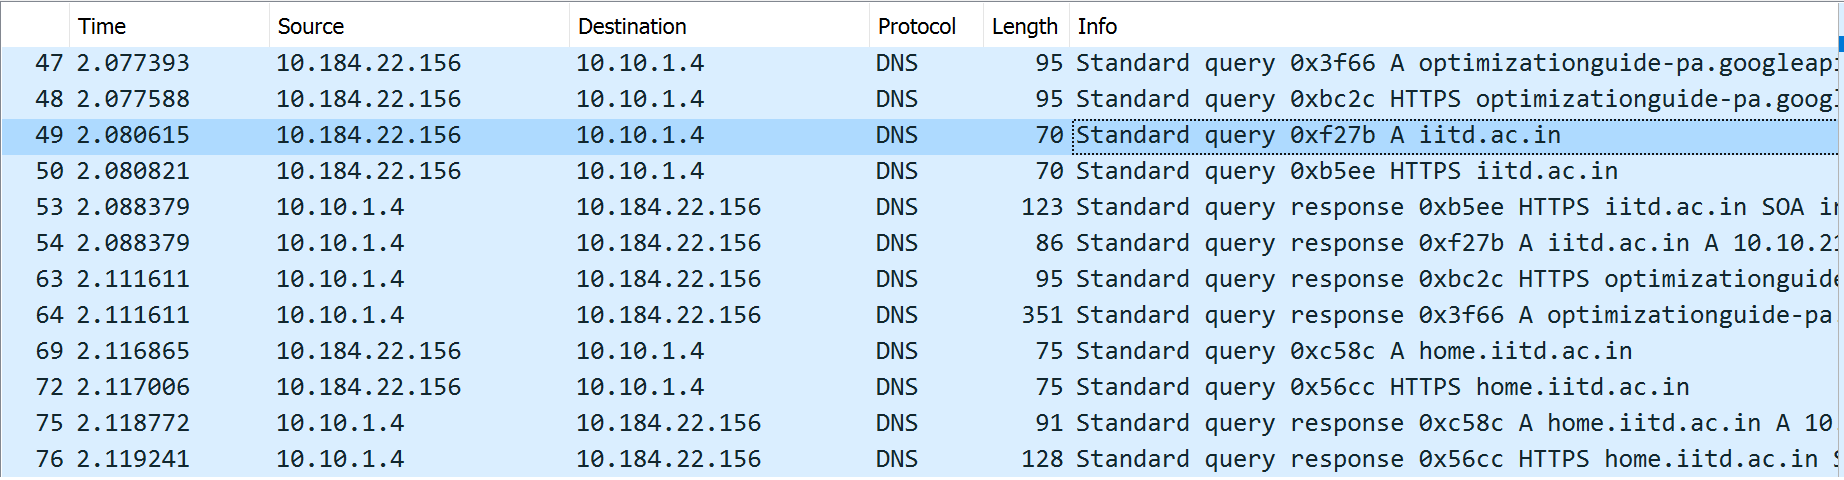
\includegraphics[scale=0.5]{images/IITD dns.png}
        \caption{IITD DNS}
        \label{fig:IITDDNS}
    \end{figure}
    \subsubsection*{Observations}
    As shown in the figure \cref{fig:IITDDNS}, we observe  there were DNS queries and responses for {\tt iitd.ac.in}. It began
\end{enumerate}
\clearpage
\section{Appendix: Preparatory Tasks}
Here, we provide information about the various tools available for network analysis

\subsection{\texttt{ifconfig/ipconfig}}
  This is used to find the following for the network interfaces on the computer:
    \begin{description}
        \item[\textit{IP address}] An IP (Internet Protocol) address is a numerical label assigned to each device connected to a computer network that uses the Internet Protocol for communication. It serves two main purposes: identifying the host or network interface and providing the location of the host in the network. IP addresses can be either IPv4 (32-bit) or IPv6 (128-bit) and are written in a dotted-decimal format (e.g., {\tt172.31.225.222} for IPv4 or {\tt fe80::215:5dff:feeb:19f7} for IPv6).
        \item[\textit{Gateway}] A gateway, often referred to as a default gateway, is a network device (usually a router) that serves as an access point to other networks. It acts as an intermediary between devices within a local network and devices on other networks, including the internet. When a device on a local network wants to communicate with a device on another network, it sends the data to the gateway, which then forwards it to the appropriate destination.
        \item[\textit{Network mask}] A network mask, also known as a subnet mask, is used in conjunction with an IP address to determine the network portion and the host portion of the address. It is a binary pattern of bits that help divide an IP address into a network address and a host address. The network mask is typically represented in decimal format as four octets (e.g., {\tt255.255.255.0} for IPv4). It is used in the process of subnetting to identify which part of the IP address identifies the network and which part identifies the individual host within that network.
        \item[\textit{Hardware address}] A hardware address, also known as a MAC (Media Access Control) address, is a unique identifier assigned to a network interface card (NIC) by its manufacturer. It is a 48-bit address expressed in hexadecimal format and is used to identify a specific device on a local network. Each NIC in the world has its own unique MAC address, allowing devices to communicate with each other at the data link layer of the networking model.
        \item[\textit{DNS server}] A DNS (Domain Name System) server translates human-readable domain names, like www.google.com, into IP addresses that machines can understand. When you enter a URL in a web browser or try to access any internet resource, your device sends a DNS query to a DNS server. The DNS server then looks up the corresponding IP address associated with the domain name and returns it to your device, allowing it to establish a connection to the desired resource.
    \end{description}
    
    Running \texttt{ifconfig} on our system connected to Wifi gives the following output:

        
    \begin{code}
    root@IdeapadAB:~# ifconfig
    eth0: flags=4163<UP,BROADCAST,RUNNING,MULTICAST>  mtu 1500
      inet 172.31.225.222  netmask 255.255.240.0  broadcast 172.31.239.255
      inet6 fe80::215:5dff:feeb:19f7  prefixlen 64  scopeid 0x20<link>
      ether 00:15:5d:eb:19:f7  txqueuelen 1000  (Ethernet)
      RX packets 149  bytes 20663 (20.6 KB)
      RX errors 0  dropped 0  overruns 0  frame 0
      TX packets 13  bytes 1006 (1.0 KB)
      TX errors 0  dropped 0 overruns 0  carrier 0  collisions 0

    lo: flags=73<UP,LOOPBACK,RUNNING>  mtu 65536
      inet 127.0.0.1  netmask 255.0.0.0
      inet6 ::1  prefixlen 128  scopeid 0x10<host>
      loop  txqueuelen 1000  (Local Loopback)
      RX packets 0  bytes 0 (0.0 B)
      RX errors 0  dropped 0  overruns 0  frame 0
      TX packets 0  bytes 0 (0.0 B)
      TX errors 0  dropped 0 overruns 0  carrier 0  collisions 0
    \end{code}

    And on running it on mobile hotspot, we get the following output:
    \begin{code}
    root@IdeapadAB:~# ifconfig
    eth0: flags=4163<UP,BROADCAST,RUNNING,MULTICAST>  mtu 1500
        inet 172.31.225.222  netmask 255.255.240.0  broadcast 172.31.239.255
        inet6 fe80::215:5dff:feeb:19f7  prefixlen 64  scopeid 0x20<link>
        ether 00:15:5d:eb:19:f7  txqueuelen 1000  (Ethernet)
        RX packets 1035  bytes 154375 (154.3 KB)
        RX errors 0  dropped 0  overruns 0  frame 0
        TX packets 103  bytes 8962 (8.9 KB)
        TX errors 0  dropped 0 overruns 0  carrier 0  collisions 0

    lo: flags=73<UP,LOOPBACK,RUNNING>  mtu 65536
        inet 127.0.0.1  netmask 255.0.0.0
        inet6 ::1  prefixlen 128  scopeid 0x10<host>
        loop  txqueuelen 1000  (Local Loopback)
        RX packets 0  bytes 0 (0.0 B)
        RX errors 0  dropped 0  overruns 0  frame 0
        TX packets 0  bytes 0 (0.0 B)
        TX errors 0  dropped 0 overruns 0  carrier 0  collisions 0
    \end{code}

    %%%%%%%%%%%%%%%%%%%%%%% Why is the ip address in both the same? %%%%%%%%%%%%%%%%%%%%%%%

    {\tt eth0} and {\tt lo} are two different network interfaces. {\tt eth0} is associated with the Ethernet connection and {\tt lo} is the loopback(localhost) interface.

    Here is a description of the various fields in the output:
    \begin{description}
        \item[\textit{flags}] A set of flags that indicate the status of the network interface. 
        \item[\textit{mtu}] The Maximum Transmission Unit (MTU) is the size of the largest packet that can be transmitted over the network interface without being fragmented. The MTU is typically measured in bytes and can range from 64 to 65535 bytes.
        \item[\textit{inet}] The IPv4 address assigned to the network interface.
        \item[\textit{netmask}] The subnet mask for the IPv4 address. It helps determine the network and host portions of the IP address.
        \item[\textit{broadcast}] The broadcast address for the network. It is used to send data to all devices on the local network.
        \item[\textit{inet6}] The IPv6 link-local address with a prefix length of 64 bits. IPv6 addresses are written in hexadecimal format and are longer than IPv4 addresses.
        \item[\textit{ether}] The unique hardware address (MAC address) of the network interface card.
        \item[\textit{txqueuelen}] The length of the transmit queue.
        \item[\textit{RX packets}] The number of received packets.
        \item[\textit{TX packets}] The number of transmitted packets.
        \item[\textit{RX errors}] The number of receive errors.
        \item[\textit{TX errors}] The number of transmit errors.
        \item[\textit{dropped}] The number of dropped packets due to errors.
        \item[\textit{overruns}] The number of packets that had data sent beyond their allowed length.
        \item[\textit{frame}] The number of packets with framing errors.
        \item[\textit{collisions}] The number of packet collisions (i.e., when two devices transmit data at the same time).
    \end{description}
    
    The IP address of the smartphone can be found by "Settings$\rightarrow$About phone$\rightarrow$Status$\rightarrow$IP address"

\subsection{\tt ping}
This is used to discover if a particular IP address is online or not. For example, in the following code we are pinging www.google.com with packets of size 10 bytes and varying the TTL. We observe that as the TTL decreases, the packet doesn't reach the destination. This is because the TTL is decremented by 1 at each hop and when it reaches 0, the packet is dropped and an ICMP error message is sent back to the source. The source then knows that the packet didn't reach the destination and hence the destination is not online.
\begin{code}
root@IdeapadAB:~# ping -c 3 -s 50 -t 10 www.google.com
PING www.google.com (142.250.195.4) 50(78) bytes of data.
58 bytes from del12s09-in-f4.1e100.net (142.250.195.4): icmp_seq=1 ttl=55 time=82.3 ms
58 bytes from del12s09-in-f4.1e100.net (142.250.195.4): icmp_seq=2 ttl=55 time=67.1 ms
58 bytes from del12s09-in-f4.1e100.net (142.250.195.4): icmp_seq=3 ttl=55 time=33.1 ms

--- www.google.com ping statistics ---
3 packets transmitted, 3 received, 0% packet loss, time 2004ms
rtt min/avg/max/mdev = 33.130/60.834/82.271/20.545 ms
root@IdeapadAB:~# ping -c 3 -s 50 -t 9 www.google.com
PING www.google.com (142.250.195.4) 50(78) bytes of data.
From 142.251.52.213 (142.251.52.213) icmp_seq=1 Time to live exceeded
From 142.251.52.213 (142.251.52.213) icmp_seq=2 Time to live exceeded
From 142.251.52.213 (142.251.52.213) icmp_seq=3 Time to live exceeded

--- www.google.com ping statistics ---
3 packets transmitted, 0 received, +3 errors, 100% packet loss, time 2299ms
pipe 2
\end{code}



\subsection{\tt traceroute}
This gives you the sequence of routers that a packet traverses to get to a particular destination.
\begin{code}
C:\Users\Anish>tracert iitd.ac.in

Tracing route to iitd.ac.in [103.27.9.24]
over a maximum of 30 hops:

1     3 ms     4 ms     3 ms  192.168.107.98
2    39 ms    29 ms    21 ms  10.50.97.29
3    54 ms    46 ms    23 ms  10.50.97.223
4    58 ms    25 ms    34 ms  10.50.97.77
5   190 ms    30 ms    46 ms  dsl-ncr-dynamic-017.24.23.125.airtelbroadband.in [125.23.24.17]
6    63 ms    37 ms    27 ms  116.119.109.76
7    51 ms    38 ms    26 ms  49.44.187.164
8     *        *        *     Request timed out.
9     *        *        *     Request timed out.
10    38 ms    27 ms    27 ms  136.232.148.178
11     *        *        *     Request timed out.
12     *        *        *     Request timed out.
13     *        *        *     Request timed out.
14    53 ms    36 ms    60 ms  103.27.9.24
15    85 ms    35 ms    36 ms  103.27.9.24
16   148 ms   101 ms    86 ms  103.27.9.24

Trace complete.
\end{code}
\subsection{\tt nslookup}
This command helps you communicate with DNS servers to get the IP address for a particular hostname.

\subsection{\tt nmap}
This is a handy network diagnostics tool that you can use to discover which hosts are online in the network, and even try to infer what operating system the hosts might be running.

\subsection{\tt wireshark}
This is a very useful tool to sniff packets on the wire (or wireless medium). Sniffed data is parsed by wireshark and presented in an easily readable format with details of the protocols being used at different layers.

\end{document}
